Eine reversible Maschine X arbeite zwischen den Temperaturen $T_\text{w} > T_\text{k}$ mit dem Wirkungsgrad $\eta_\text{X}$, der ideale Stirlingmotor mit $\eta_\text{S}$. Der ideale Stirlingmotor ist ebenfalls reversibel: Rückwärts betrieben ist er eine ideale Wärmepumpe, die mit der Arbeit $W$ dem warmen Reservoir die Wärme $W/\eta_\text{S}$ zuführt.

Angenommen, es wäre $\eta_\text{X} > \eta_\text{S}$. Die Maschine X entzieht dem warmen Reservoir die Wärme $Q$ und verrichtet die Arbeit $W = \eta_\text{X}\,Q$. Mit dieser Arbeit treiben wir den Stirlingmotor rückwärts als Wärmepumpe an.
\begin{center}
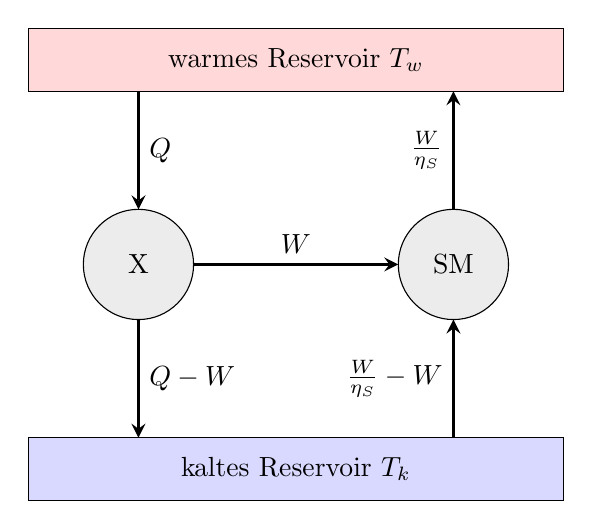
\begin{tikzpicture}[>=stealth]
 \draw[fill=red!15] (-3.4,2.2) rectangle (3.4,3.0);
 \node at (0,2.6) {warmes Reservoir $T_\text{w}$};
 \draw[fill=blue!15] (-3.4,-2.2) rectangle (3.4,-3.0);
 \node at (0,-2.6) {kaltes Reservoir $T_\text{k}$};
 \draw[fill=gray!15] (-2,0) circle (0.7);
 \node at (-2,0) {X};
 \draw[fill=gray!15] (2,0) circle (0.7);
 \node at (2,0) {SM};
 \draw[->, very thick] (-2,2.2) -- (-2,0.7) node[midway, right] {$Q$};
 \draw[->, very thick] (-2,-0.7) -- (-2,-2.2) node[midway, right] {$Q-W$};
 \draw[->, very thick] (-1.3,0) -- (1.3,0) node[midway, above] {$W$};
 \draw[->, very thick] (2,-2.2) -- (2,-0.7) node[midway, left] {$\frac{W}{\eta_\text{S}}-W$};
 \draw[->, very thick] (2,0.7) -- (2,2.2) node[midway, left] {$\frac{W}{\eta_\text{S}}$};
\end{tikzpicture}
\end{center}
Die Wärmepumpe gibt dem warmen Reservoir die Wärme
\begin{align}
 \frac{W}{\eta_\text{S}} &= \frac{\eta_\text{X}}{\eta_\text{S}}\,Q > Q
\end{align}
zurück. Beide Maschinen zusammen arbeiten periodisch, verrichten netto keine Arbeit und transportieren nur die Wärme $\left(\frac{\eta_\text{X}}{\eta_\text{S}}-1\right)Q > 0$ vom kalten zum warmen Reservoir. Das widerspricht dem zweiten Hauptsatz (Clausius). Also ist $\eta_\text{X} \leq \eta_\text{S}$.

Weil auch X reversibel ist, kann man die Rollen vertauschen: Der Stirlingmotor treibt die rückwärts laufende Maschine X an. Dasselbe Argument liefert $\eta_\text{S} \leq \eta_\text{X}$. Zusammen folgt
\begin{align}
 \eta_\text{X} &= \eta_\text{S} = 1-\frac{T_\text{k}}{T_\text{w}}
\end{align}
Jede reversible, periodisch zwischen $T_\text{w}$ und $T_\text{k}$ arbeitende Maschine hat also den Carnot-Wirkungsgrad. (Für eine irreversible Maschine gilt nur der erste Schritt: $\eta \leq \eta_\text{S}$.)
